\imprimircapa

\imprimirfolhaderosto*

\begin{fichacatalografica}
    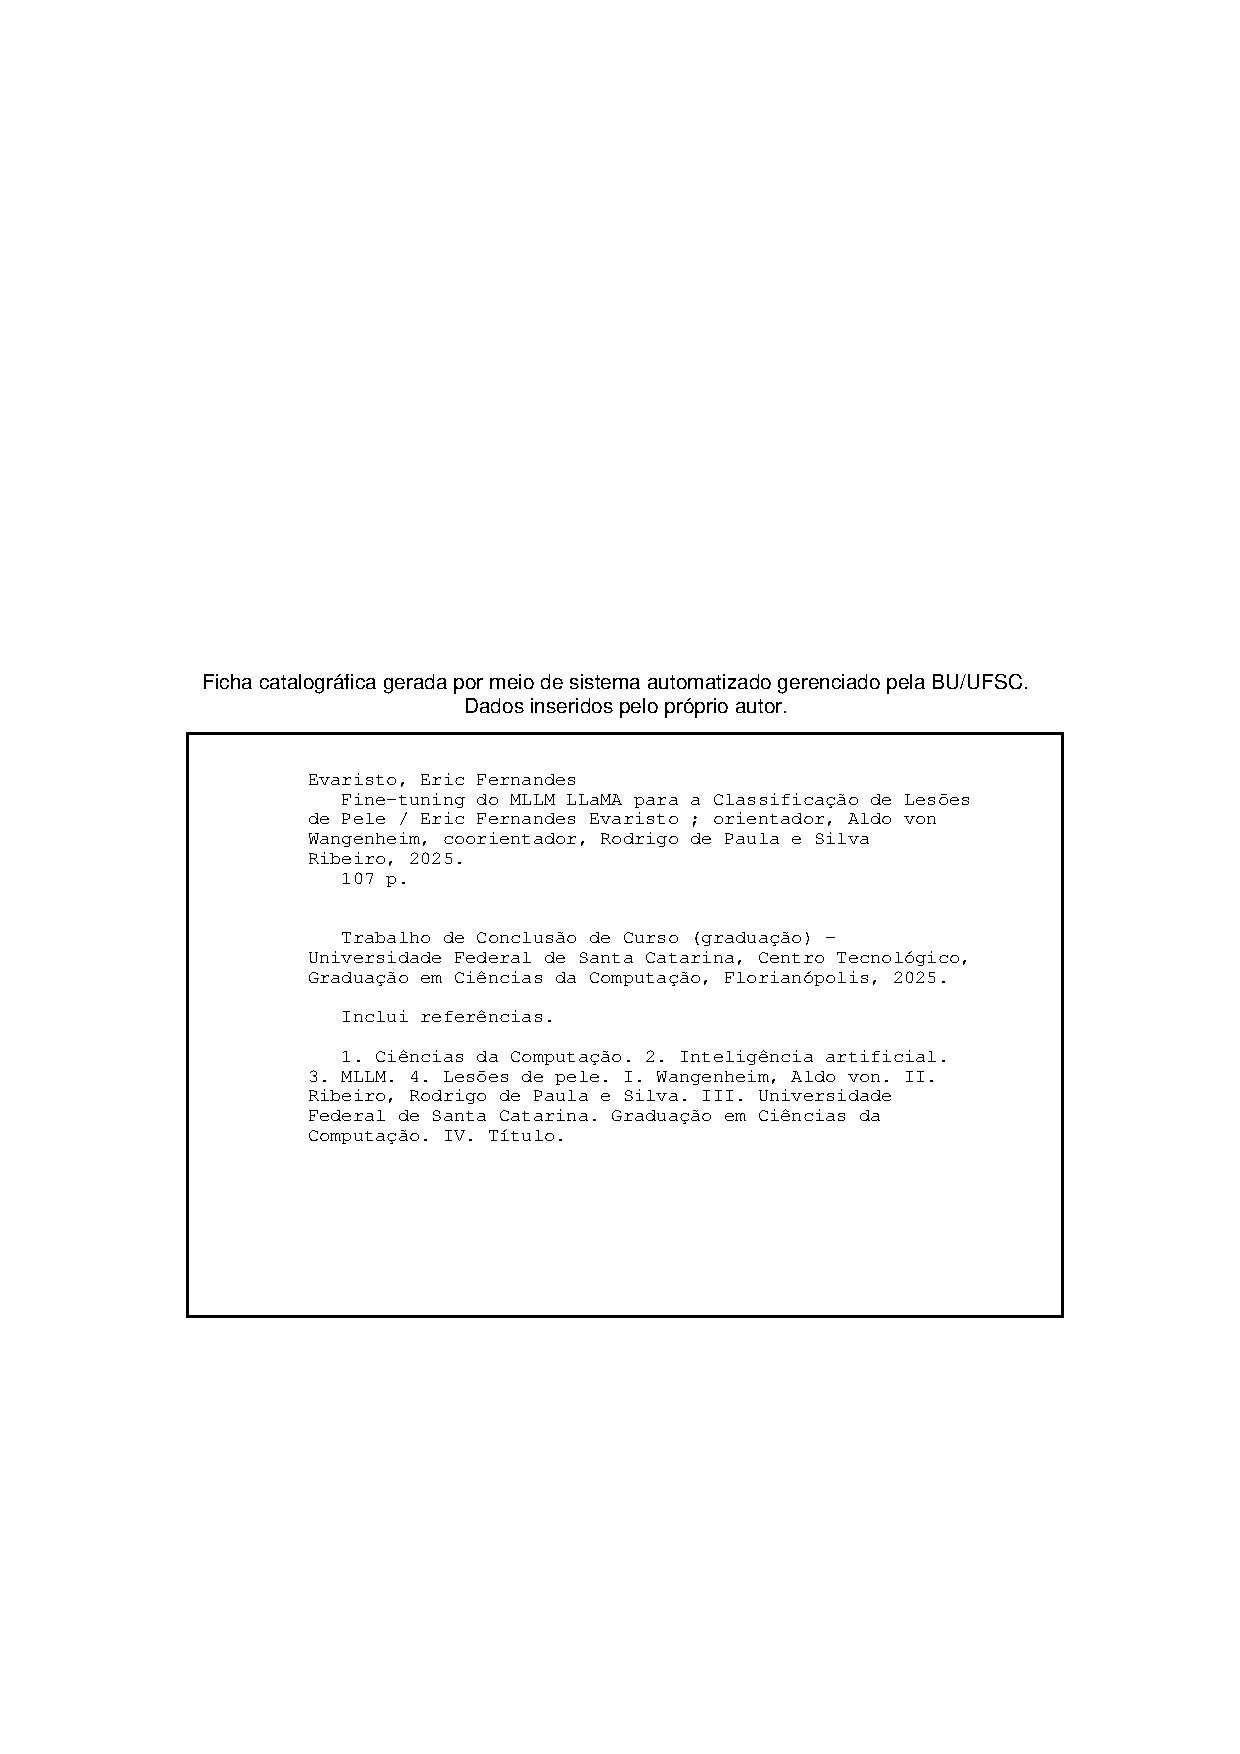
\includepdf{beforetext/Ficha_Catalografica.pdf}
\end{fichacatalografica}

\begin{folhadeaprovacao}
    \begin{center}
        {\imprimirautor}

        \begin{center}
            \ABNTEXchapterfont\bfseries\MakeUppercase{\imprimirtitulo}\ifnotempty{\imprimirsubtitulo}{:
            \imprimirsubtitulo}
        \end{center}

        \begin{minipage}{\textwidth}
            Este Trabalho de Conclusão de Curso foi julgado adequado para obtenção do Título de
            Bacharel em Ciências da Computação e aprovado em sua forma final pelo Curso de Graduação em Ciências da
            Computação do Departamento de Informática e Estatística (INE), Centro Tecnológico (CTC) da Universidade
            Federal de Santa Catarina (UFSC).
        \end{minipage}
    \end{center}

    \imprimirlocal, 11 de junho de 2025.

    \assinatura{
    \textbf{\imprimircoordenador} \\
    Coordenadora do Curso
    }

    \vspace{1cm}
    \textbf{Banca Examinadora:}

    \vspace{1cm}
    \assinatura{
    	\textbf{\imprimirorientador} \\
		\imprimirorientadorRotulo \\
		\imprimirinstituicao
    }

    \vspace{1cm}
    \assinatura{
		\textbf{\imprimircoorientador} \\
		\imprimircoorientadorRotulo \\
		\imprimirinstituicao
    }

    \vspace{1cm}
    \assinatura{
	    \textbf{Harley Miguel Wagner, MSc.} \\
		\imprimirinstituicao
    }
\end{folhadeaprovacao}

\begin{agradecimentos}
    Primeiramente, agradeço à minha mãe, Marly, e ao meu pai, Joacir, por me incentivarem sempre na busca pelo
    conhecimento e por me proporcionarem a oportunidade de chegar até aqui. Sem seus esforços, compreensão e amor, este
    trabalho não seria possível. Agradeço também aos meus avós, Gracinha e Izaltino (\textit{in memoriam}), e a todos
    os outros familiares que me acompanharam ao longo da vida.

    Aos meus amigos do curso, agradeço pelo apoio e pelos bons momentos no decorrer da graduação. Em especial, à
    Gabriela, por estar ao meu lado tanto nos dias felizes quanto nos difíceis, sempre me dando apoio. Agradeço também
    aos meus amigos das engenharias e da vida por me acompanharem nesta jornada.

    Agradeço também ao Aldo e ao Rodrigo pela orientação e valiosas recomendações que ajudaram no desenvolvimento deste
    trabalho. Agradeço também ao grupo de pesquisa de MLLMs e a todos que participaram da produção dos trabalhos
    científicos que fundamentaram este trabalho.

    Agradeço ao Laboratório Bridge, em especial à equipe Legacy, pelo apoio e incentivo.

    Também agradeço à equipe Protto UFSC, pelo acolhimento no início da graduação e pelas aventuras em áreas diferentes
    da computação.

    Expresso também minha gratidão à UFSC e a todos os professores e servidores que deram o seu melhor para oferecer um
    curso de ciências da computação de qualidade.
\end{agradecimentos}


\setlength{\absparsep}{18pt}
\begin{resumo}
    \SingleSpacing
    Lesões de pele podem ser um indicador de diversas doenças, incluindo as graves, como o câncer de pele. A detecção
    precoce dessas lesões é fundamental para o tratamento e a cura da doença. No entanto, o diagnóstico preciso só pode
    ser feito por profissionais qualificados, como dermatologistas.

    Uma parte do atendimento de atenção primária no Brasil é feita por \ac{ACS}. Estes profissionais estão em contato
    direto com a população, porém, não são qualificados para realizar a triagem de casos de lesões de pele.
    Considerando este cenário, uma ferramenta capaz de classificar lesões de pele e também fornecer pré-diagnósticos e
    recomendações seria de grande utilidade.

    \acp{MLLM} possuem as capacidades necessárias para o desenvolvimento de uma ferramenta como esta, pois podem
    classificar imagens e gerar descrições textuais com base no seu conteúdo. Além disso, estes modelos podem ser
    adaptados para tarefas específicas através de \textit{fine-tuning}.

    Com o objetivo de avaliar o uso de um \ac{MLLM} para a classificação de lesões de pele e a geração de laudos, foi
    realizado neste trabalho o \textit{fine-tuning} do \ac{LLaMA} 3.2 11B com as técnicas \ac{QLoRA} e \ac{LoRA}, ambas
    baseadas em \ac{PEFT}. O desenvolvimento foi realizado em duas etapas. Na primeira, o conjunto de imagens de
    dermatoscopia \ac{HAM10000} foi utilizado no \textit{fine-tuning} do modelo para apenas classificar lesões de pele.
    Nesta fase, o melhor modelo foi treinado com \ac{QLoRA} e obteve uma acurácia de 87,4\%. Na etapa final, um
    conjunto de imagens de aproximação, proveniente do \ac{STT/SC}, foi utilizado no \textit{fine-tuning} para a
    classificação de lesões e geração de laudos. O modelo final treinado com \ac{QLoRA} e apresentou uma acurácia de
    45,2\%, enquanto o modelo com \ac{LoRA} obteve 44,5\%. O baixo desempenho dos modelos finais na classificação pode
    ser explicado por inconsistências no conjunto de dados.

    \textbf{Palavras-chave}: Lesões de pele. Câncer de pele. MLLM. LLaMA. PEFT. Fine tuning. QLoRA. LoRA.
\end{resumo}

\begin{resumo}[Abstract]
    \SingleSpacing
    \begin{otherlanguage*}{english}
        Skin lesions can be an indicator of several diseases, including serious ones like skin cancer. The early
        detection of these lesions is fundamental for the treatment and cure of the disease. However, an accurate
        diagnosis can only be made by qualified professionals, such as dermatologists.

        Part of the primary care service in Brazil is carried out by \acf{ACS}. These professionals are in direct
        contact with the population, however, they are not qualified to perform the screening of skin lesion cases.
        Considering this scenario, a tool capable of classifying skin lesions and also providing pre-diagnoses and
        recommendations would be of great use.

        \acfp{MLLM} have the necessary capabilities for the development of a tool like this, as they can classify
        images and generate textual descriptions based on their content. Furthermore, these models can be adapted for
        specific tasks through fine-tuning.

        With the objective of evaluating the use of an \ac{MLLM} for the classification of skin lesions and the
        generation of reports, this work carried out the fine-tuning of \acf{LLaMA} 3.2 11B with the \acf{QLoRA} and
        \acf{LoRA} techniques, both based on \acf{PEFT}. The development was carried out in two stages. In the first,
        the \acf{HAM10000} dermatoscopy image dataset was used in the fine-tuning of the model to only classify skin
        lesions. In this phase, the best model was trained with \ac{QLoRA} and obtained an accuracy of 87.4\%. In the
        final stage, a set of close-up images, from \acf{STT/SC}, was used in the fine-tuning for the classification of
        lesions and generation of reports. The final model trained with QLoRA presented an accuracy of 45.2\%, while
        the model with \ac{LoRA} obtained 44.5\%. The low performance of the final models in the classification can be
        explained by inconsistencies in the dataset.

        \textbf{Keywords}: Skin lesions. Skin cancer. MLLM. LLaMA. PEFT. Fine-tuning. QLoRA. LoRA.
    \end{otherlanguage*}
\end{resumo}

{
\hypersetup{hidelinks}

\pdfbookmark[0]{\listfigurename}{lof}
\listoffigures

\imprimirlistadesiglas

\pdfbookmark[0] {
\contentsname}{toc}
\tableofcontents*
\cleardoublepage
}
